Support Vector Machines (SVM) are often called the large margin classifiers because SVM try to separate learning data with the highest possible margin~\citep{article:fletcher}. By separating classes in the training data with a high margin, it will obtain a better accuracy when classifying unobserved instances. Basically, SVM can only classify binary problems, however by dividing the problem into several subclassifications, SVM can be used for multi-class tasks also.

\begin{figure}[ht]
	\begin{minipage}[b]{0.45\linewidth}
		\centering
		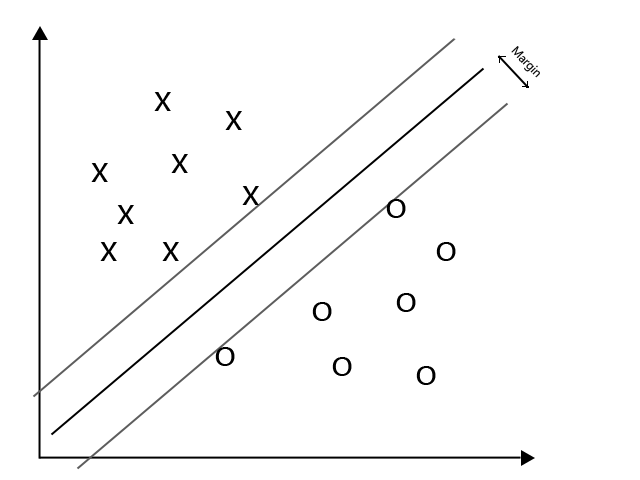
\includegraphics[width=\textwidth]{figs/linear.png}
		\caption{The hyperplane linearly separates the data into two classes. The points closest to the hyperplane are the support vectors.}
		\label{fig:linear}
	\end{minipage}
	\hspace{0.5cm}
	\begin{minipage}[b]{0.45\linewidth}
		\centering
		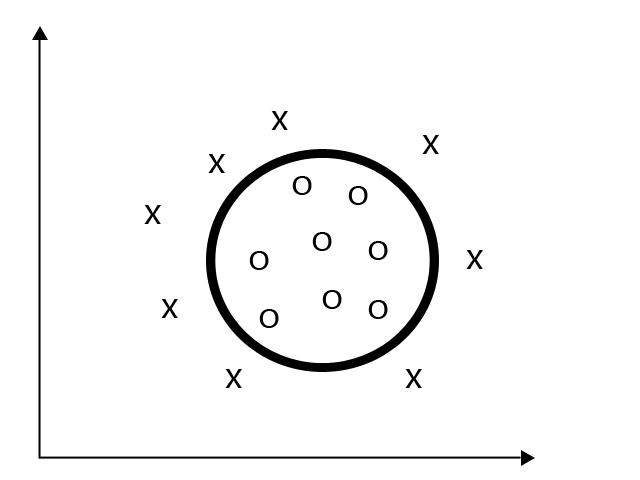
\includegraphics[width=\textwidth]{figs/non-linear.png}
		\caption{An example of a non-linear problem. A kernel function is used to map these data points into a higher dimensional feature space.}
		\label{fig:non-linear}
	\end{minipage}
\end{figure}

The equation for the separating hyperplane is defined by the closest points to the margin, as seen in~\autoref{fig:linear} These points are called \emph{support vectors}. In cases where the data is non-linear, as in~\autoref{fig:non-linear}, a kernel function is used to project the data into a high-dimensional space where it is linearly separable.
